\section{Příklad 2}
% Jako parametr zadejte skupinu (A-H)
\druhyZadani{E}

Principem Théveninova teorému je, že složitý obvod nahradíme obvodem náhradního skutečného zdroje napětí (tedy ideálním zdrojem napětí a odporem představujícím jeho vnitřní odpor), ke kterému je připojena zátěž. Poté je triviální spočítat napětí na této zátěži a proud jí procházející.

V tomto případě je zátěží rezistor $R_6$. Cílem postupu je získat náhradní napětí $U_x$ a náhradní odpor $R_x$ podle obrázku \ref{fig:circ-2-1}. Překreslíme obvod bez zátěže:
\begin{figure}[H]
    \centering
    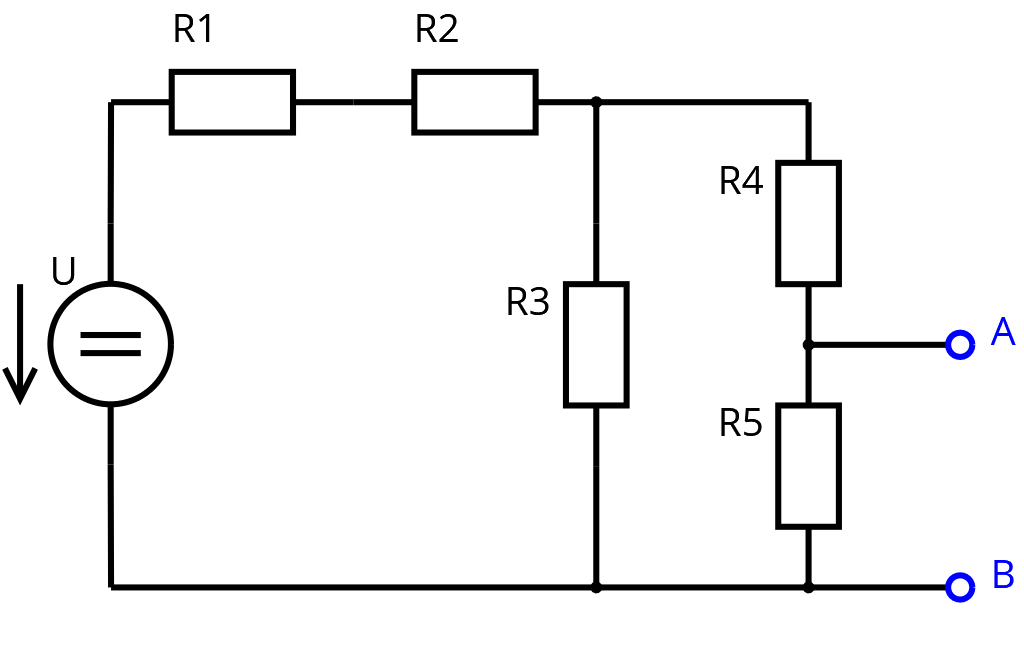
\includegraphics[width=7cm]{diagrams/Diagram5.png}
    \caption{Obvod bez zátěže, která je nahrazena svorkami \textcolor{blue}{A}, \textcolor{blue}{B}.}
    \label{fig:circ-2-1}
\end{figure}

Náhradní odpor $R_x$ vypočítáme tak, že jediný napěťový zdroj původního obvodu nahradíme zkratem a spočítáme odpor mezi svorkami \textcolor{blue}{A} a \textcolor{blue}{B}. Na obrázku \ref{fig:circ-2-2} je zakreslen stav po nahrazení zdroje, na obrázku \ref{fig:circ-2-3} je pak vzniklá odporová síť překreslena, aby bylo zřejmé, jakým způsobem je možné její celkový odpor vypočítat.
\begin{figure}[htb]
    \centering
    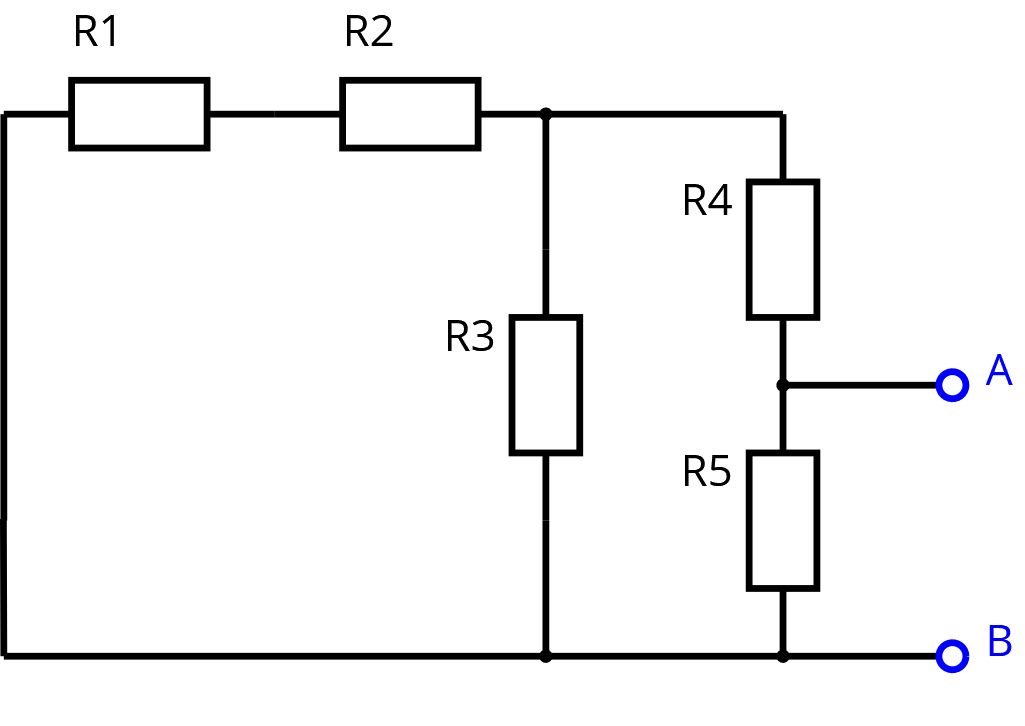
\includegraphics[width=7cm]{diagrams/Diagram6.png}
    \caption{Obvod po nahrazení napěťového zdroje zkratem.}
    \label{fig:circ-2-2}
\end{figure}
\begin{figure}[htb]
    \centering
    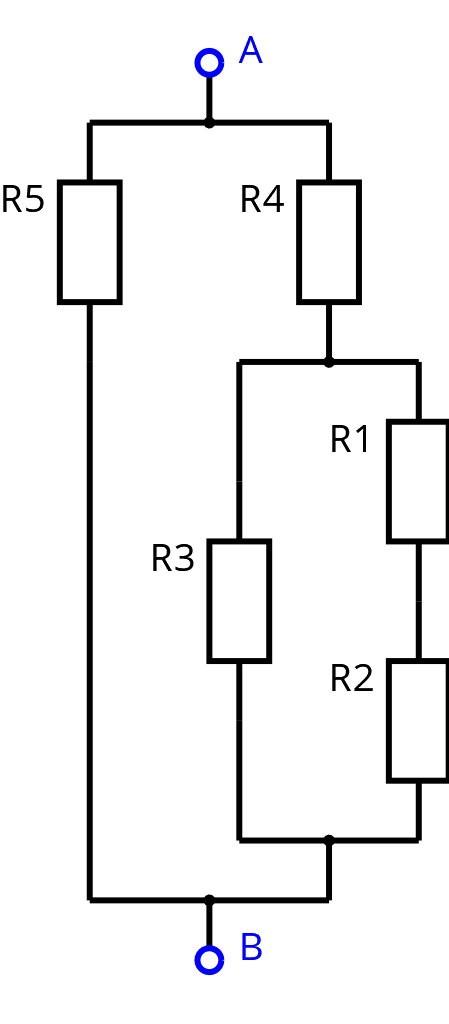
\includegraphics[height=7cm]{diagrams/Diagram7.png}
    \caption{Překreslený obvod z obrázku \ref{fig:circ-2-2}.}
    \label{fig:circ-2-3}
\end{figure}

Odpor mezi svorkami vypočítáme postupným zjednodušováním sítě:
\begin{gather*}
    \frac{1}{R_x} = \frac{1}{R_5} + \frac{1}{R_{1234}} = \frac{1}{R_5} + \frac{1}{\displaystyle R_4 + \frac{R_{12} R_3}{R_{12} + R_3}} = \frac{1}{R_5} + \frac{1}{\displaystyle R_4 + \frac{(R_1+R_2)R_3}{R_1 + R_2 + R_3}} \\
    R_x = \frac{1}{\displaystyle \frac{1}{600} + \frac{1}{245 + \frac{(150+335)\cdot 625}{150 + 335 + 625}}} \\
    \\
    \mathbf{R_x \approx \SI{278.0211}{\ohm}}
\end{gather*}

Napětí náhradního zdroje $U_x$ spočítáme jako napětí mezi svorkami \textcolor{blue}{A}, \textcolor{blue}{B} v~obvodu bez zátěže, jde o~tzv.~\textit{napětí naprázdno}. Z obrázku \ref{fig:circ-2-1} je zřejmé, že napětí mezi svorkami se bude rovnat napětí na rezistoru $R_5$. (Z logiky věci, při pohledu na zadání je vidět, že $R_5$ a $R_6$ jsou dva paralelně spojené rezistory, na kterých se dělí proud, ale napětí je stejné.) Spočítáme $U_{R_5}\ (=U_x)$ opět metodou zjednodušování. Popisované veličiny jsou naznačeny v obrázku \ref{fig:circ-2-4}.
\begin{figure}[htb]
    \centering
    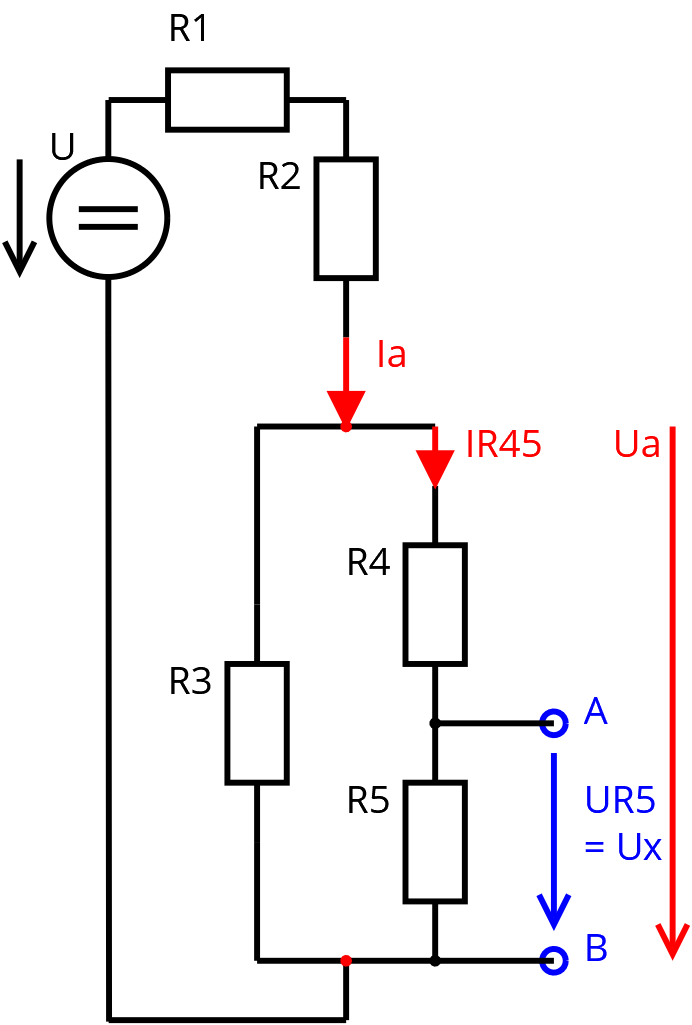
\includegraphics[height=10cm]{diagrams/Diagram8.png}
    \caption{Hledané proudy a napětí pro zjištění napětí naprázdno.}
    \label{fig:circ-2-4}
\end{figure}
\begin{gather*}
    I_a = \frac{U}{R_{ekv}} \\
    R_{ekv} = R_1 + R_2 + \frac{R_3(R_4+R_5)}{R_3+R_4+R_5} \\
    U_a = U - I_a(R_1 + R_2) \\
    U_{R_5} = I_{R_{45}} R_5 = \frac{U_a}{R_{45}} R_5 = U_a \frac{R_5}{R_4+R_5} = \left[U - \frac{U}{R_{ekv}}(R_1+R_2)\right]\frac{R_5}{R_4+R_5} \\
    U_{R_5} = U \frac{R_3 R_5}{(R_1+R_2)(R_3+R_4+R_5)+R_3(R_4+R_5)} \\
    \\
    \mathbf{U_x = U_{R_5} \approx \SI{75.5394}{\volt}}
\end{gather*}

Zjistili jsme, že náhradní skutečný zdroj bude mít napětí $U_x=\SI{75.5394}{\volt}$ a vnitřní odpor $R_x=\SI{278.0211}{\ohm}$. Pro původní obvod tak můžeme vytvořit ekvivalentní obvod, jaký je uveden na obrázku \ref{fig:circ-2-5}. Snadno pak spočítáme napětí $U_{R_6}$ na zátěži a proud $I_{R_6}$ jí procházející.
\begin{figure}[H]
    \centering
    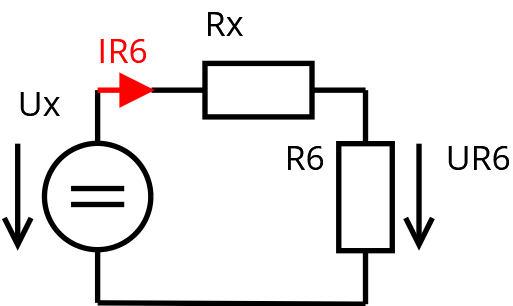
\includegraphics[width=4.5cm]{diagrams/Diagram9.png}
    \caption{Ekvivalentní obvod.}
    \label{fig:circ-2-5}
\end{figure}
\begin{gather*}
    I_{R_6} = \frac{U_x}{R_x+R_6} \\
    I_{R_6} = \frac{\num{75.5394}}{\num{278.0211}+150} \\
    \mathbf{I_{R_6} \approx \SI{0.176485}{\ampere} = \SI{176.485}{\milli\ampere}} \\
    \\
    U_{R_6} = I_{R_6} R_6 \\
    U_{R_6} = \frac{\num{75.5394}\cdot 150}{\num{278.0211}+150} \\
    \mathbf{U_{R_6} \approx \SI{26.4728}{\volt}}
\end{gather*}